\documentclass{llncs}
\usepackage{fullpage}

%load needed packages
\usepackage{graphicx}
\usepackage{array}
\usepackage{booktabs}
\usepackage[utf8]{inputenc}


\begin{document}

\title{Práctica 1}

\author{Fernando Luis Pinilla Molina \\ Hugo Herrero González \\ Ignacio Freijeiro Tapia \\ Alfonso Ramos Rojas}
\institute{\email{fernan925@uma.es \\hugohg@uma.es \\ nacho.freijeiro@uma.es \\ alfonsram@uma.es } \\
Aprendizaje Automático. Universidad De Málaga.}



\maketitle 

\vspace{0.5cm} % Space down the title

\textit{
Esta práctica introduce el uso de Python y sus librerías esenciales para el aprendizaje automático (NumPy, Pandas, Matplotlib, Scikit-learn). Siguiendo un ejemplo previo con el dataset Iris, aplicamos operaciones similares de exploración de datos, cálculo estadístico, visualización y entrenamiento de un modelo simple sobre el dataset de Cáncer de Mama de Wisconsin, disponible en Scikit-learn.}

\section{Introducción}
El proyecto se centra en el análisis exploratorio y posterior aplicación de un modelo de aprendizaje automático sobre el conjunto de los datos de Breast Cancer Wisconsin. El dataset es un recurso estándar que se usa en Machine Learning para los problemas de clasificación binaria.
Nuestro objetivo principal es predecir si la masa celular mamaria es Maligna o no Benigna, las indicamos con la etiqueta 0 o 1 respectivamente. Para predecir cual es cada una nos basamos en características digitalizadas de las muestras clínicas.

\vspace{0.5cm}


\section{Conclusiones Gráficas}

\subsection{Histograma de Radio Medio}

Este histograma ilustra la distribución de frecuencias de la característica \textbf{radio medio} (el radio promedio de los núcleos celulares) en el conjunto de datos de \textit{Cáncer de Mama}. \vspace{0.2cm}

El eje X representa los valores del radio medio, mientras que el eje Y indica la frecuencia, es decir, cuántas muestras (tumores) presentan un radio medio dentro de cada intervalo (\textit{bin}).\vspace{0.2cm}

Se observa que la mayoría de las muestras tienen un radio medio concentrado entre aproximadamente \textbf{10 y 15}, con la frecuencia más alta (más de 175 muestras) situándose en el intervalo alrededor de los valores \textbf{12–13}. \vspace{0.2cm}

La distribución presenta un \textbf{sesgo hacia la derecha} (asimetría positiva), indicando que hay menos muestras con radios medios muy grandes (por encima de 20), pero estos valores más altos extienden la cola de la distribución en esa dirección.

\vspace{0.3cm}
\noindent
Los datos estadísticos proporcionados complementan esta visión:

\begin{itemize}
    \item \textbf{Media del radio medio:} 14.13
    \item \textbf{Mediana:} 13.37 
    
    El hecho de que la media sea ligeramente superior a la mediana es consistente con el sesgo a la derecha observado en el histograma.
    \item \textbf{Desviación típica:} 3.52, la cual cuantifica la dispersión o variabilidad de los valores del radio medio alrededor de la media.
\end{itemize}

\noindent
En resumen, el histograma muestra que los \textbf{radios medios más pequeños y medianos son los más comunes} en las muestras, con una disminución progresiva en la frecuencia a medida que el radio medio aumenta.


\begin{figure}
	\centering
	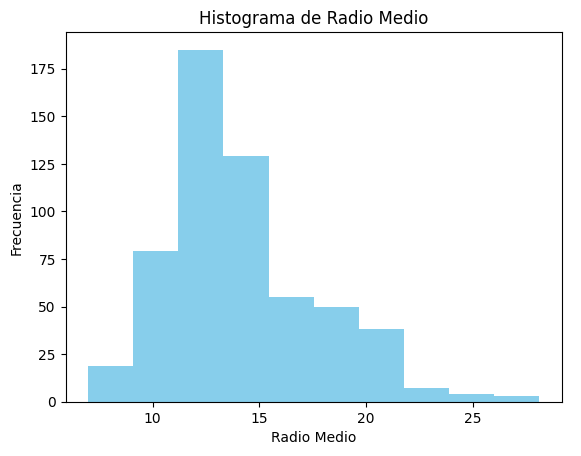
\includegraphics[width=0.50\textwidth]{images/Histograma de Radio Medio.png}
	\caption{Histograma del radio medio}
	\label{fig:1}
\end{figure}


\subsection{Dispersión por tipo de tumor}
La gráfica \ref{fig:2} nos muestra la correlación entre el Radio Medio y la Textura Media. Cada punto que nos aparece nos representa una muestra, y usamos la codificación por color según la clase de tumor que sea:
\begin{itemize}
	\item Maligno: Color rojo
	\item Benigno: Color Verde
\end{itemize}
De la gráfica podemos extraer diferentes conclusiones sobre la separación de los datos.
\begin{enumerate}
\item \textbf{Separación de clases:} Podemos observar que los tumores benignos se agrupan en la región de los valores bajos para el radio medio y la textura media, mientras que los tumores malignos se agrupan en la región de los valores más altos para el radio medio y la textura media.
\item \textbf{Utilidad:} También vemos que el radio medio es muy efectivo para la separación, ya que los puntos con un radio medio pequeño son casi excluvivamente benignos, y los puntos con un radio medio grande son mayoritariamente malignos.
\item \textbf{Región de Ambigüedad: } Podemos ver en la gráfica que tenemos una región de ambigüedad, principalmente en la zona central. En el área esta, vemos que las muestras de ambas clases se comienzan a mezclar, lo que nos indica que una clasificación perfecta usando solo estas dos variables sería prácticamente imposible y nos generaría los pocos errores de clasificación que podemos ver en la matriz de confusión.
\end{enumerate}
\clearpage
\begin{figure}
	\centering
	\includegraphics[width=0.30\textwidth]{images/Dispersión por tipo de tumor.png}
	\caption{Dispersión por tipo de tumor}
	\label{fig:2}
\end{figure}

\subsection{Número de tumores por clase}

En la gráfica podemos ver que tenemos más casos de tumores benignos que malignos, por lo que el conjunto de datos presenta un desequilibrio de clases que puede influir en los resultados de los modelos predictivos. Por ello, podría ser recomendable aplicar alguna técnica de balanceo de datos.

\begin{figure}
	\centering
	\includegraphics[width=0.30\textwidth]{images/Número de tumores por clase.png}
	\caption{Número de tumores por clase}
	\label{fig:3}
\end{figure}

\subsection{Gráfica comparación medidas}

En esta gráfica podemos observar que tanto el radio medio como la textura media son menores en los casos benignos, esto puede indicarnos que los tumores malignos tienden a ser más grandes y a tener una estructura más heterogénea en su textura. Es decir, podemos concluir que existe una relación clara entre las características físicas del tumor y su naturaleza(maligna o benigna).
\clearpage

\begin{figure}
	\centering
	\includegraphics[width=0.30\textwidth]{images/Comparación de medidas promedio por clase.png}
	\caption{Comparación de medidas promedio por clase}
	\label{fig:4}
\end{figure}
\subsection{Radio Medio por clase}
Sobre el análisis de las medias con respecto a la clase en la gráfica \ref{fig:radio_medio_clase}:
\begin{itemize}
	\item Los tumores malignos tienen una dispersión de valores mucho mas grande que los benignos
	\item Los tumores malignos presentan un radio medio (17.5cm) muy superior al de los benignos (12.5cm).
\end{itemize}


\begin{figure}
	\centering
	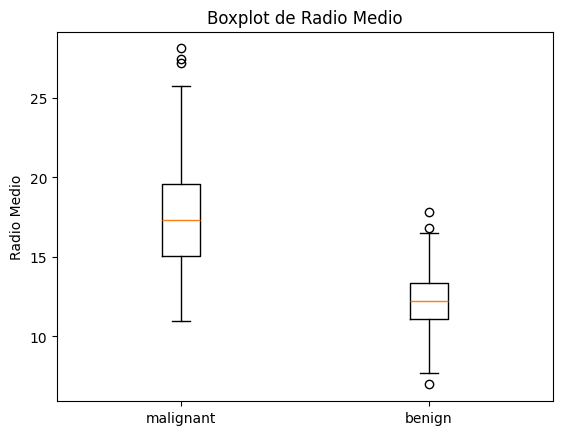
\includegraphics[width=0.30\textwidth]{images/Boxplot de Radio Medio.png}
	\caption{Boxplot del radio medio}
	\label{fig:radio_medio_clase}
\end{figure}

\section{Conclusiónes Modelo}

Para terminar esta práctica hemos generado un modelo predictivo simple usando clasificación por árbol de decisión, para ello, primero hemos usado parte del conjunto de datos para entrenamiento y luego hemos usado el resto de datos para evaluar su rendimiento.

Hemos obtenido una precisión


\begin{figure}
	\centering
	
\includegraphics[width=0.30\textwidth]{images/uma_logo.jpg}
	\caption{Logo de la universidad}
	\label{fig:logo_uma}
\end{figure}

\end{document}

